%%%%%%%%%%%%%%%%%%%%%%%%%%%%
% Two Sword Lengths Apart
% Christopher Gandrud
% 21 July 2013
%%%%%%%%%%%%%%%%%%%%%%%%%%%%

% !Rnw weave = knitr

\documentclass[a4paper]{article}\usepackage[]{graphicx}\usepackage[]{color}
%% maxwidth is the original width if it is less than linewidth
%% otherwise use linewidth (to make sure the graphics do not exceed the margin)
\makeatletter
\def\maxwidth{ %
  \ifdim\Gin@nat@width>\linewidth
    \linewidth
  \else
    \Gin@nat@width
  \fi
}
\makeatother

\definecolor{fgcolor}{rgb}{0.345, 0.345, 0.345}
\newcommand{\hlnum}[1]{\textcolor[rgb]{0.686,0.059,0.569}{#1}}%
\newcommand{\hlstr}[1]{\textcolor[rgb]{0.192,0.494,0.8}{#1}}%
\newcommand{\hlcom}[1]{\textcolor[rgb]{0.678,0.584,0.686}{\textit{#1}}}%
\newcommand{\hlopt}[1]{\textcolor[rgb]{0,0,0}{#1}}%
\newcommand{\hlstd}[1]{\textcolor[rgb]{0.345,0.345,0.345}{#1}}%
\newcommand{\hlkwa}[1]{\textcolor[rgb]{0.161,0.373,0.58}{\textbf{#1}}}%
\newcommand{\hlkwb}[1]{\textcolor[rgb]{0.69,0.353,0.396}{#1}}%
\newcommand{\hlkwc}[1]{\textcolor[rgb]{0.333,0.667,0.333}{#1}}%
\newcommand{\hlkwd}[1]{\textcolor[rgb]{0.737,0.353,0.396}{\textbf{#1}}}%

\usepackage{framed}
\makeatletter
\newenvironment{kframe}{%
 \def\at@end@of@kframe{}%
 \ifinner\ifhmode%
  \def\at@end@of@kframe{\end{minipage}}%
  \begin{minipage}{\columnwidth}%
 \fi\fi%
 \def\FrameCommand##1{\hskip\@totalleftmargin \hskip-\fboxsep
 \colorbox{shadecolor}{##1}\hskip-\fboxsep
     % There is no \\@totalrightmargin, so:
     \hskip-\linewidth \hskip-\@totalleftmargin \hskip\columnwidth}%
 \MakeFramed {\advance\hsize-\width
   \@totalleftmargin\z@ \linewidth\hsize
   \@setminipage}}%
 {\par\unskip\endMakeFramed%
 \at@end@of@kframe}
\makeatother

\definecolor{shadecolor}{rgb}{.97, .97, .97}
\definecolor{messagecolor}{rgb}{0, 0, 0}
\definecolor{warningcolor}{rgb}{1, 0, 1}
\definecolor{errorcolor}{rgb}{1, 0, 0}
\newenvironment{knitrout}{}{} % an empty environment to be redefined in TeX

\usepackage{alltt}
\usepackage{fullpage}
\usepackage{lscape}
\usepackage[authoryear]{natbib}
\usepackage{setspace}
    \doublespacing
\usepackage{hyperref}
\hypersetup{
    colorlinks,
    citecolor=black,
    filecolor=black,
    linkcolor=cyan,
    urlcolor=cyan
}
\usepackage{booktabs}
\usepackage{dcolumn}
\usepackage{url}
\usepackage{tikz}
\usepackage{todonotes}
\usepackage{verbatim}
\usepackage{endnotes}


\setlength{\belowcaptionskip}{0.5cm}

%%%%%%% Title Page %%%%%%%%%%%%%%%%%%%%%%%%%%%%%%%%%%%%%%%%%%%%
\title{Two Sword Lengths Apart: Violence in Multi-party Elected National Legislatures}

\author{Christopher Gandrud \\
                {\emph{Hertie School of Governance}}\footnote{Research Associate. Friedrichstra{\ss}er 180. 10117 Berlin, Germany. Email: \href{mailto:christopher.gandrud@gmail.com}{christopher.gandrud@gmail.com}. Thank you to Emily Beaulieu, Gary Cox, Simon Hix, and seminar participants at Yonsei University for very helpful comments. I would also like to thank Hortense Badarani for excellent research assistance and my students at the LSE for inspiration. An earlier version was circulated under the title ``Two Sword Lengths: Losers' consent and violence in national legislatures''.}}
\IfFileExists{upquote.sty}{\usepackage{upquote}}{}
                
\begin{document}

\maketitle

%%%%%%% Abstract %%%%%%%%%%%%%%%%%%%%%%%%%%%%%%%%%%%%%%%%%%%%
\begin{abstract}
Multi-party elected national legislatures should be venues for peacefully resolving conflicts between opposing groups. However, they can sometimes become the scenes of physical violence between legislators. Such violence is an indication that a country's legislative institutions are functioning far from perfectly as legislative actors are deciding to drop out of the normal rules of the `game'. In this first global study of legislative violence, I argue that violence is often the result of credible commitment problems where legislators find it difficult to credibly commit to follow peaceful bargaining outcomes, including non-violent legislative rules. The problem is exacerbated when legislatures are unfair. Unfairness is higher and the credible commitment problems more acute in countries with disproportionate electoral outcomes and new democracies. I find robust evidence for this argument using a case study of legislative violence in the antebullum United States Senate and a new global data set of incidence from the 1980s through Winter 2011.
\end{abstract}


\paragraph{Keywords:} legislatures, violence, credible commitment problems, fairness, electoral proportionality, institutional design, majority and minority governments

\vspace{0.3cm}

%%%%%%% Introduction %%%%%%%%%%%%%%%%%%%%%%%%%%%%%%%%%%%%%%%%%%%%

Though legislators in democracies are often described as `battling' or `fighting' we expect these battles to be in terms of rhetoric and procedural manoeuvres, circumscribed by non-violent rules, that culminate in votes. The outcomes of these contests are then respected by all legislators. However, metaphorical battles sometimes become physical fights between members of legislatures. 

The histories of many legislative chambers contain incidents of violence between legislators. In 1856 a member of the United States House of Representatives canned a senator unconscious in the Senate chamber \citep{USSenateCanning}. It has been suggested that the United Kingdom's House of Commons is physically designed to prevent violence between members. The Government and Opposition benches are said to be ``two sword lengths apart" \citep{ParliamentUKSword} so that duels will be fought with words rather than swords. Actual, sword fights do not seem to have taken place in the Commons chamber, but violent incidences did occur. For example, in 1893 a fight broke out between Irish nationalist and Unionist members of parliament \citep{ByrneViolence}. Violence in legislatures continues to occur, with incidences being regularly reported on by the media.\endnote{The Guardian newspaper, for example, sporadically compiles stories of physical fights in legislative chambers. See \url{http://www.guardian.co.uk/politics/gallery/2010/dec/17/1\#/?picture=369861052\&index=0}. Legislative violence has also has its own Wikipedia page. See {\url{http://en.wikipedia.org/wiki/Legislative_violence}}.} Recent instances of violence between legislators include multiple brawls in Ukraine in 2010 and South Korea in 2009. In both cases opposition legislators, facing impending legislative defeats, tried to obstruct the governments' attempts to pass controversial legislation.\endnote{In Ukraine the fight was over Russian military bases and in South Korea it concerned media ownership laws.} Even more recently in 2013 a large confrontation occurred in the Venezuelan National Assembly when the Assembly President withheld speaking time from legislators who did not recognized the victory of the new president in a very highly contested election.

Until recently legislative disruption, of which violence is an extreme form, has largely been ignored by political scientists.\endnote{A recent special issue of \emph{Democratization} \citeyearpar{Democratization2013} entitled \emph{Disruptive Democracy: Analysing Legislative Protest} has made a persuasive case that it deserves scholarly attention. Indeed, these acts reflect ``political conflict as well as systemic issues in democratic and democratizing institutional contexts'' \citep[394-395]{Spary2013}.} Though non-violent legislative disruption is not necessarily `good' or `bad' \citep[see][for discussions of how non-violent disruption may act as a  `safety valve']{Ostrow1996,Young2002}, legislative violence is a dramatic break from scholars' assumption that compliance with legislative rules of the `game' is a given \citep{Wolfe2004} and as such symbolizes poorly functioning legislative institutions. Some single-country case study work has been done on--mostly non-violent--legislative disruption \cite[see][]{Armitage2013,Johnson2013,Ilie2013,Wolfe2004} and other work has examined the strategic and expressive choices politicians make when they decide to not participate in the democratic rules of the game \citep[e.g.][]{wilkinson2006,Beaulieu2008,Spary2013,BeaulieuForthcoming}. In this paper I extend this work by advancing a theory of legislative violence in multi-party elected national legislatures and test it using both case study and global-level data. Indeed, this paper includes the first cross-country description of violence between legislators. 

I begin the paper by advancing an argument for understanding when legislative violence between members in multi-party elected legislatures is more likely. I argue that violence is often the result of credible commitment problems where legislators find it difficult to credibly commit to follow peaceful bargaining outcomes, including non-violent legislative rules. As with international conflict, credible commitment problems can make disruption and violence more attractive options for pursuing legislative goals than peaceful bargaining, because the commitments that result from bargaining are incredible. I propose that when members of a parliament\endnote{Unless mentioned otherwise, I use `legislature' and `parliament' interchangeably.} view their legislature as unfair, credible commitment problems will be greater and therefore the probability of violence higher. At least two observable factors are very important for determining fairness and the likelihood that commitments will be adhered to: the \emph{proportionality of a country's electoral outcomes} and the \emph{age of its democracy}. After proposing this argument and discussing a number of key alternative explanations, I begin to empirically examine the argument with a case study of the 1856 canning of US Senator Charles Sumner. I then move to a global level study of contemporary legislative violence by describing a new data set of incidences from 1981 through Winter 2011. In this section I also demonstrate simple associations between my argument's key variables and violence on a global scale. I then discuss the variables and rare event logistic regression models \citep{KingRareEvents2001, KingRareEventsPA2001} I use to further study these rare events. Finally, I lay out my parametric model evidence that legislative violence is more prevalent in countries with disproportionate electoral outcomes and in new democracies. I also find that violence is more likely in legislatures with small minority governments. I conclude the paper with a discussion of the possible implications of these findings for designers of democratic institutions and directions for future research.

%%%%%%%%%%%%%%%%%%%%%%%%%%%%%%%%%%%%%%%%%%%%%% Previous Research & Framework

\section{Understanding Legislative Violence: Credible Commitment Problems and Fairness}

Legislative violence, like other forms of disruption, can be used for both strategic \citep[see][]{Beaulieu2008,BeaulieuForthcoming} and expressive or performative \citep[see][]{Rai2013,Spary2013} purposes by both legislative winners and losers. Legislative losers--those who are not in control of the ``legislative cartel''  that sets the agenda \citep{cox2007} and are not part of the deciding majority--may use violence to stall legislation or rule changes they dislike. Winners--those in the legislative cartel--could use violence to prevent losers from utilizing procedures that might constrain their decision-making power. Both winners and losers may use violence to shore up support among their proponents \citep{wilkinson2006}, as a way of expressing dissatisfaction with legislative outcomes, and to publicize issues they and their supporters care about \citep{Spary2013}. Winners may not only use active violence, but also might make a strategic choice not to use their powers, e.g. control of security forces, to prevent or curtail losers' violence \citep[see the work on ethnic violence in India by][]{wilkinson2006} with the hope that losers will be publicly discredited. This is certainly not an exhaustive list of the ways legislators interact with one another and can use violence to achieve strategic and expressive ends, but instead illustrates many of them.

\subsection{A Theory of Legislative Violence}

Just because actors can gain a strategic advantage or express their discontent through violence does not mean they will choose to. This is indicated by the relatively rare incidences of legislative violence across the world. In my global sample there are 88 incidents from 1981 through Winter 2011. Just as violence may have strategic and expressive benefits, it also entails costs. There are physical costs of conflict. There may be penalties imposed on violent legislators, such as prohibitions on entering the chamber or holding committee positions. Violent legislators may suffer reputational costs. Non-violent legislative rules prescribe `appropriate behavior' \citep{March2008}. Violence is `inappropriate' and as such could damage a legislator's reputation. 

The expected utility of violence may be low, as violence may not be a very effective way to actually achieve legislative goals, at least to the extent that it can be used to stop unwanted legislation. For example, in the Ukrainian and Korean examples mentioned above, the controversial legislation was passed despite the use of violence intended to stall it. Echoing a fundamental question in international relations: if violence is costly and has a low expected utility, why does it happen at all? 

Further drawing on the international relations literature, I argue that violence in multi-party elected legislatures is often the result of the inability of legislators to credibly commit to follow peaceful bargaining outcomes, including non-violent legislative rules. \cite{Fearon1995} argued that when actors are not able to make credible commitments violent conflict between states is more likely \cite[see also][]{Powell2006}. If it is difficult to believe that a peaceful bargaining outcome will actually happen because bargained commitments will likely be broken, actors will choose violence to achieve their goals. We can extend this logic to legislatures. In multi-party elected legislatures winners and losers--who may some day become a winners--need to be able to credibly commit to not simply use or remake legislative procedures in only their narrow self-interest. They need to commit to limits on their power \citep{riker1982,Gaubatz1996}, especially legislative rules and procedures that are the result of peaceful bargaining processes. If they are not able to credibly make these commitments then legislators may come to believe that disruption and violence is the best way to achieve their goals, despite its general costs and low expected utility. What makes legislative credible commitment problem more or less severe? 

Credible commitment problems are generally smaller and therefore violence is less likely when legislators in multi-party elected legislatures view parliament's procedures and their implementation as fair. I define fairness as \emph{the degree to which seats in the legislature and legislative resources, such as speaking time and committee appointments, proportionally correspond to voters' support}. I argue that unfairness increases legislative credible commitment problems in at least two ways: it creates possibilities for shifts in power from those who benefit from unfair legislatures to beneficiaries of more fair systems and prevents fairness equilibria.

Unfair legislatures have the possibility for large and rapid shifts in legislative power from those who benefit from the unfair rules to those that would benefit from fairer rules. For example, if an electoral system that creates disproportionate outcomes becomes more proportional, then the winning parties may be likely to change over the course of one election. The new winners could then further alter legislative procedures to benefit themselves. \cite{Powell2004} identified major commitment problems in situations with large and rapid power shifts. We can apply his logic to legislatures. Temporarily weak legislators--those with disproportionally fewer seats and access to legislative resources under unfair rules--who are not in the legislative cartel need to `buy off' those that are temporarily strong--the beneficiaries of the unfair legislature in the cartel--in order to avoid the strong further dramatically changing the rules to benefit themselves. Buying off in this context may simply mean agreeing to continue rules that make the legislature unfair at the status quo level. However, because the presently weak have the potential to be much stronger, they are likely to renege on agreements that disproportionately benefit the temporarily strong. They may also have an incentive to use disruption or violence to prevent further unfair rule changes or indeed force the rules to become fairer to actively increase their power. The temporarily strong may use disruption or violence to prevent the rules from becoming fairer.

Why would highly proportional electoral systems not create equally large credible commitment problems for legislators that would benefit from a large increases in unfairness? In other words, why would a fair legislature create an equilibrium? Rabin's \citeyearpar{Rabin1993} work studying bargaining consequences when actors care about fairness in addition to material well-being provides an answer. Because actors care about fairness, they are more likely to maintain commitments (punish defectors), even if it hurts their material well-being, when others are being fair (unfair). One form of punishment could be reputational damage inflicted in fair systems by both supporters and opponents of violent legislators who care about fairness. This reduces legislators' incentives to defect from fair rules and bargains even if they could gain legislative power by increasing unfairness. As such credible commitment problems are lower and actors can reach a ``fairness equilibrium''. Experimental research has supported the idea that commitments are more credible if they are more fair \citep{Ellingsen2004} and can even act as an enforcement device for incomplete contracts \citep[see][for a review]{Fehr2008}. 

\subsection{Observing Situations Where Credible Commitment Problems are Worse?}

To empirically test my theory I focus on two easily observable factors that could strongly influence legislators' fairness and credible commitment problems: proportionality of electoral outcomes and age of democracy.

\paragraph{Proportional Electoral Outcomes}

Possibly the most important and easily observable component of legislature fairness is the proportionality of the election that allocated its seats and therefore the control of its procedures. Disproportional, i.e. unfair, electoral outcomes create credible commitment problems as they create the potential for shifts in power from beneficiaries of unfair to fair rules. More proportional systems conversely enable fairness equilibria. At what observable levels of disproportionality would we expect to see more violence? At most levels of disproportionality there may be credible commitment problems of some degree, because there will be legislators who benefit for an increase in proportionality. It is only when outcomes are close to perfectly proportional that the gains from increasing proportionality are very small or virtually none existent. At the same time in systems with very proportional electoral outcomes it is easy for all to identify the electoral outcomes as fair, thus enabling fairness equilibria.\endnote{When their is ambiguity over how fair the system is actors may not impose very high costs, such as reputational damage, from breaking the rules.} Because of this we should not expect a linear relationship between disproportionality and violence. There should instead be a threshold effect where very proportional electoral systems will have very low levels of violence due to very small or non-existent credible commitment problems. 

Recent empirical research on the functional form of the relationship between political trust and disproportionality provides some initial evidence for the claim that there could be a threshold effect between disproportionality and legislative violence. \cite{Marien2011} found that there was a curvilinear relationship between proportional electoral outcomes and citizens' political trust. Feelings of political trust were highest with very proportional outcomes\endnote{The most trusting societies had Gallagher disproportionality scores around 1. See the discussion below for further details about this measure.} as well as disproportional or majoritarian systems. Countries in the middle had the lowest trust.\endnote{Outcomes in the middle may be a ``bastard-producing hybrid'' \citep[74]{Sartori1994} that combines the defects of both highly proportional and disproportional outcomes.} Marien argues that high trust in very proportional systems is caused by high fairness. The fairness effect seems to quickly disappear as we move in the direction of more disproportionate outcomes. Marien argues that high voter trust in very disproportionate countries is caused not by fairness, but by high accountability.\endnote{Disproportional majoritarian elections produce highly accountable legislatures where citizens feel a strong sense of control over their politicians \citep{Aarts2008,CHO2012}.} So should we expect a similar curvilinear relationship between proportionality and legislative violence? Probably not. Though accountability may please voters in general, there is little reason to believe that this will ameliorate the credible commitment problems created by unfairness.

For these reasons \emph{we should expect countries with very proportional outcomes have lower incidences of violence. All other countries should be more likely to have relatively more violence.} 

It's important to note that though the exact type of electoral system is ultimately interesting to us from an institutional design point of view, we should not confuse ``the outcome of an electoral system with its mechanics" \citep[][109]{Golder2005}.\endnote{How proportional an outcome is can be affected by both electoral system rules and the distribution of party support within a country, for example.} When studying how elections influence the propensity of losers to use legislative violence we are more interested in how proportional electoral outcomes are, rather than the exact type of electoral system that produced these outcomes. 

\paragraph{New vs. Old Democracies}

Legislators in older democracies are more likely to view their parliament as fair and are more likely to be able to make credible commitments. There are a number of reasons for this. In new democracies, as with political regime change in general, the rules of the game are in flux. This can give present winners considerable power to set the rules to their advantage. The first actors to gain power after a transition--who may represent a disproportionately small segment of the electorate--may be better able to establish unfair rules, entrenching their power \cite[108]{Saideman2002}, before the democratic regime has fully consolidated. This could lead to credible commitment problems between the temporarily strong that are making the rules during the democratic transition and the temporarily weak who could gain more if the rules were fairer. 

Also, in the relatively early days of a democracy the legislative party system may be shifting considerably \cite[see][161 for a review]{Mainwaring2007b},\endnote{\cite{Mainwaring2007b} argue that it is the time period when democracy was created that is associated with party volatility rather than the number of years a country is democratic. However, their analysis they base this claim on is highly problematic because (a) they arbitrarily limit the democracy years variable to 30, ruling out effects beyond 30 years and (b) include this variable in the same models as the highly correlated democratic age variable which can lead to unreliable coefficient estimates.} possibly as politicians work out electoral coordination problems \citep[e.g.][]{cox1997}. New democracies may also have rapidly changing economies and demographics that further change the party system and the proportionality of legislative rules. Even if initial rules were fair when the legislative rules were created, they may quickly become less so as the country changes. On average, these shifts could be much larger in new as opposed to old democracies. As we will see in the antebellum US example below, large rapid demographic and party system shifts dramatically altered the fairness of the distribution of power in the US Senate between pro and anti-slavery senators around the 1840s and 1850s. Because of the instability of new party systems, there is a greater likelihood that legislatures could become unfair leading to credible commitment problems and violence.

The alternation of power that generally occurs as democratic regimes survive longer gives legislators more information about the credibility of others' commitments. In new democracies actors simply may not have gathered enough information to know if they can someday become winners. Losers in new democracies may not have learned that ``pretenders to office can expect to reach it, losers can expect to come back" \citep[][36]{Przeworski1991}. Actual alternations of power allow legislators to gather better information about the credibility of commitments to allow fair alternations of power. Increased information about others' abilities to make credible commitments could strengthen the credibility of future commitments, thus reducing violence.

There may also be a survivor bias created as democracies age. If legislatures are unable to overcome credible commitment problems in some way, legislative institutions will not function as a way to peacefully organize bargaining. This could lead to discontent and social unrest both inside and outside of the legislature, possibly leading to democratic collapse. New democracies unable to overcome credible commitment problems simply would not survive long enough to become old.

For these reasons we should expect to see that \emph{violence is more common in new democracies' legislatures.}

\section{Alternative Explanations}

The usefulness of an argument can be partially judged by how well it explains events compared to major alternative explanations. What alternative factors may explain instances of legislative violence across countries?

\paragraph{The Size of the Governing Majority}

The use of legislative procedures may be viewed as more legitimate and therefore worth following simply if there are larger proportions of the parliament supporting them, i.e. if the governing majority is larger. However, the relationship between the size of the governing legislative majority and violence is not clear cut \emph{ex ante}. 

On the one hand is the proposition that, though far from the only way of thinking about democratic legitimacy \cite[see][for a discussion]{Follesdal2006}, majority rule is a foundational concept of democracy \citep{Dahl1989} and an important component of democratic legitimacy. An extensive literature led by Arend Lijphart makes the argument that perceptions of democratic legitimacy are larger as the proportion of actors involved in decision-making increases \citep[see][]{Lijphart2007}. The more legislators that are involved in parliamentary decision-making, the more likely it is that legislators will view procedures as legitimate and worth following. 

On the other hand another causal mechanism may be at work if there is a relative lack of violence in legislatures with very large majorities. Perhaps these majorities are simply so powerful that they can quickly quash legislative disruption before it starts or even prevent serious opposition politicians becoming legislators to begin with. These sorts of actions may be less likely in the types of legislatures that are the focus of this paper--multi-party elected legislatures--, though they are certainly not impossible. 

We also have good reasons to suspect that very large legislative majorities may actually increase the incidences of violence in democratic legislatures. If a parliament has a large hegemonic party, minority politicians may feel marginalized. They may have no way to influence policy-making other than with extreme acts of legislative disruption, like violence.

What about at the other end of the spectrum? Minority governments are often constrained in their ability to pass legislation by themselves. They need to assemble a coalition of opposition politicians in order to pass legislation. Though the official legislative cartel has a minority of the seats, legislation still requires a majority to pass (depending on the voting rules). However, this does not necessarily mean that we should expect no difference in how minority and majority governments are perceived as fair and the size of credible commitment problems. Though they may be constrained in their ability to pass legislation without the support of other parties, they can still wield considerable power over the parliamentary agenda, such as by restricting plenary speaking time \citep{Tsebelis2002,cox2005,cox2007}. Though it is often difficult to determine the exact issue legislative fights are over (in many cases there are multiple overlapping issues) many instances do involve disagreements over control of the agenda. The recent Venezuelan example mentioned above, for instance involved a conflict over conditions that the governing majority was placing on speaking time. Other legislators may be very inclined to view a minority government's agenda control as unfair and see opportunities to increase their power by changing the rules. As such future credible commitments would be more difficult to make and violence would be more likely. 

\paragraph{Legislative Immunity \& Violence}

There is an important institutional design feature that might directly prevent violence. Like in society generally, having laws that outlaw violence and sanction violators of these laws may dissuade physical attacks. In many countries legislators are immune from prosecution or at least arrest in the legislative chamber. Such immunity is often granted in order to prevent the legislature from being harassed and obstructed by the executive or judicial branches of government  \citep{Seghetti1984}. However, legislators immune from legal consequences may be more likely to physically harass and obstruct one another. Legislators who do not have this immunity might be less likely to attack their colleagues. 

It's important to note that if legislative violence is created by credible commitment problems, where legislators are not able to commit to peaceful bargains and rules, then it is unlikely that they would be prevented from using violence due to a lack of immunity. At the best a lack of immunity would make violence more costly thus marginally decrease credible commitment problems, but not eliminate them. Furthermore, since the ``application of punishment is inherently political'', formal rules may not have any deterrent effect if legislators do not believe they will be applied to them for political reasons \cite[58]{Wolfe2004}.

\paragraph{Culture}

Some have argued that certain regional cultures are less likely to respect democratic institutions. If this is true, then these cultures might be more likely to have legislative violence. The many popular hypotheses about East Asian cultures\endnote{These are often referred to as `Confusion' cultures \citep{Inglehart2005, Inglehart2010}.} and democratic instability are especially relevant for us given the high number of brawls in East Asia, notably in Japan, South Korea and Taiwan (see Figure \ref{leg_map}). One view is that Asian societies have hierarchical and deferential cultures that are incompatible with democracy because authority is valued over self-expression \citep[see][212-213 for a discussion]{Dalton2005}. It is unclear how this hypothesis would explain the high frequency of legislative violence in Asian democracies. It would seem to actually suggest less violence. Recent empirical evidence has found that Asian societies are in fact not strongly deferential to authority, especially when compared to Western ones \citep{Dalton2005, KimAsianValues2010}. Mostly using Inglehart and Welzel's World Values Survey data, \cite{KimAsianValues2010} actually finds that East Asian societies have lower respect for authority than non-Asians and South-east Asians. Assuming that societal values are generally congruent with legislators' values, perhaps legislators in East Asian countries are more violent because their members do not respect legislative authorities. Legislative violence in this cultural region would thus simply be the result of the same cause as violence in other low-respect for authority societies.

This and any piece of research examining the effect of political characteristics and culture on conflict face an endogeneity problem when trying to determine how they are related \citep[][751]{Carey2000}. There is an old tradition in political science \citep[][528--529]{Frye1997} arguing that culture influences institutional choice \citep[in particular see][]{Almond1963}. For example, certain cultures may be more consensual and are therefore likely to adopt consensus institutions \citep[][22-23]{Lijphart2003} including proportional electoral systems that often result in proportional outcomes. They may also be more likely to have long standing democracies. Relationships between these factors and violence could be spurious. Consensual societies may choose certain institutions and also be less violent in general, resulting in less violence between legislators. Consensual institutions may then reinforce consensual cultures and so on. These are not issues I can definitively solve here. Instead we should at least be mindful of them especially when drawing conclusions from the following analysis.

\section{Case Study: The Canning of Senator Sumner}

The breakdown of the ability to make credible commitments in unfair and new democratic legislatures is illustrated by the canning of United States Senator Charles Sumner in 1856. The development of the Senate prior to the Civil War, and especially in the 1850s, was preoccupied with the fairness of the apportionment of pro and anti-slavery senators. Two senators were elected by each state's legislature. From the end of the Revolutionary War there had been more slave states than free states and thus more slave state senators. However, compromises that were made after the Revolution to create at least as many slave states as free states, and thus as many pro-slavery as anti-slavery senators, became increasingly unfair. As the 1800s progressed these compromises were undermined by three shocks that were largely exogenous from the national legislature. The shocks created considerable opportunities for politicians from free states to increase their power by increasing fairness. The shocks were (a) factor endowments in potential new states, (b) population growth in free states, and (c) the expansion of the franchise to non-property owning white males.  The westward expansion of the United States from the 1850s posed a problem for maintaining commitments to have at least as many senators from slave as free states: there were more potential free states than slave states. This was largely the result of the fact that areas west of eastern Texas\endnote{Admitted as a slave state in 1845.} lacked land conducive to supporting plantations and the institutions of slavery \cite[see][]{Ramsdell1929,Sokoloff2000}.\endnote{Pro-slavery advocates did attempt to change the course of US expansion with the Ostend Manifesto in 1854 that promoted the annexation of Cuba as a slave state. This suggests that expansion may be endogenous to the legislative game. However, the manifesto was largely in response to a previous realization that Westward expansion which had been supported by pro-slave Democrats had actually destabilized old commitments.} Rapid population increases, partially from immigration and industrial expansion, in free states greatly increased the disproportionality of the US Senate as each free state's number of senators remained the same despite their increased population.\endnote{Industrial and population expansion in free states may have been largely the result of lacking slave institutions \citep[see][]{Sokoloff2000}. However, this dynamic is still largely exogenous of the US national legislative process. The Know Nothing party's (see below) anti-Catholic focus was in some sense a reaction to immigration from Ireland and Germany. However, this occurred after the increase in immigration began.} Many of these new people were newly eligible to vote. Between the late 1700s and the 1850s all of the states--who had the power to decide who could vote--removed almost all of their property qualifications.

Anti-slavery supporters became very vocal about this increasing unfairness. They regularly used the terms ``slave power'' and ``slavocracy'' to refer to pro-slavery advocates' disproportionate power \citep{richards2000}. For example, a friend of Congressman Horace Mann wrote to him in 1850 that ``I have been astonished for many years to see how the Slave power (not one fiftieth part of the voters) manage to control the whole United States'' \citep[quoted in][6]{Gara1969}. Gara argues that beyond concerns of the morality of slavery, ``the main thrust of [abolitionists'] attack was against slave power'' \citeyearpar[6]{Gara1969}. This concern was partially electorally motivated. Large portions of the electorate, such as white labor--who were afraid of competing with essentially free slave labor--were also concerned with slave power, though not necessarily the immorality of slavery. 

The increasing unfairness of slave power in the Senate made it difficult for anti-slavery proponents to commit to the rules of the chamber as well as credibly agree to further entrench unfair `slave power'. If they succeeded in changing the rules so that the chamber was more fair their power would increase dramatically. Also, because the arrangement was viewed as very unfair by anti-slavery politicians and a wide group of their supporters, they had lower reputational costs if they used legislative disruption. As we will see they had electoral incentives to push the boundaries of accepted legislative rules. They had far more to gain from breaking and changing the rules than following them.

\cite{Pierson1995} argues that Republican and anti-slavery proponent Charles Sumner was doing just this when he gave his May 1856 ``The Crime Against Kansas'' speech in the Senate. The speech broadly concerned the need to admit Kansas as a free state. Admitting Kansas as a free state would have resulted in a Senate that was majority free state for the first time.\endnote{California was admitted as a free state in 1850, but committed to sending one pro and one anti-slavery senator to Congress.} The speech included a number of personal attacks on pro-slavery senators, multiple allusions to slavery as rape, and denunciations of `slave power'.\endnote{For example: ``It is the rape of a virgin Territory, compelling it to the hateful embrace of Slavery; and it may be clearly traced to a depraved desire for a new Slave State, hideous offspring of such a crime, in the hope of adding to the power of Slavery in the National Government.''} This speech only barely stayed within the Senate's rules of polite discourse, especially its prohibitions of discussions of sex (a number of Democratic senators argued that it actually had broken these rules). Pierson contends that, rather than being purely emotional and personal, the speech was the culmination of an electorally motivated strategy to push the boundaries of the Senate's rules. Early in his first Senate term beginning in 1851 Sumner spoke ``within the rhetorical restraints imposed by his minority position in the Senate as well as the minority status of his own [Free Soil then Republican] party'' \cite[534]{Pierson1995}. In the early to mid 1850s party alignments shifted considerably, especially following the collapse of the Whig party in 1852.\endnote{The whigs had been divided on the issue of slavery} The new Republican party\endnote{Created in 1854.} and anti-Catholic Know Nothing party\endnote{Created in 1845.} were left to compete for the allegiance of voters who were both anti-Catholic and anti-slave power. Sumner attempted to appeal to these voters, not by attacking the Know Nothings as bigoted as some of his fellow Republicans had tried unsuccessfully to do, but by rhetorically emphasizing the problem of unfair slave power. He increased his rhetoric, pushing the bounds of Senate rules to gain more publicity for the Republican's anti-slave power position.   

The canning of Charles Sumner was in response to his Crime Against Kansas speech.\endnote{It was committed by Representative Preston Brooks, the nephew of Senator Andrew Butler, who Sumner had insulted in the speech. Representative Laurence Keitt aided the attack by using a pistol to threaten other senators who wanted to help Sumner \citep{Donald2009}.} Why? The Senate's unfairness not only made it difficult for minority anti-slavery senators to commit to the rules, it also made it difficult for the majority pro-slavery Democrats as well. They clearly did not view Republican's commitments to the unfair status quo rules as credible. They also had a lot to lose from changes that increased Senate proportionality. Rather than being a personal attack, Pierson argues that Preston Brooks' canning was ``approved by most of the Democratic party both in anticipation of and following the attack'' \cite[553]{Pierson1995}. The Democratic party's denunciation of Sumner's speech on moral grounds (especially the allusions to rape) and Brooks' subsequent attack on Sumner three days after the speech were ``designed to halt an escalation of anti-slavery rhetoric'' in the press \cite[553]{Pierson1995}. Rather than suffering reputational damage, Sumner and Brooks gained popularity among their supporters. For example, apparently ``ladies of the South would send [Brooks] hickory sticks, with which to chastise Abolistionists'' \cite[255]{Donald2009}.  

Senator Sumner's rule stretching speech and his subsequent canning happened because of an inability of the two sides to commit to follow established Senate rules and peacefully bargain on new ones. Because of increasing unfairness caused by exogenous shocks both had more to gain from disruption and violence. 

\paragraph{A Natural Experiment}

The bicameral nature of the US Congress gives us a natural experiment to further evaluate if unfairness created credible commitment problems that resulted in violence. Disproportionality increased dramatically in the US Senate because of population growth in free states and would have been further exacerbated by admission of new low population Western states as slave states (if they had been able to support slavery). However, this was not as pressing of a problem in the House of Representatives. Seats in the House are largely apportioned by population rather than state. This allowed the House to maintain a relatively constant level of proportionality even as the number of states increased and populations grew in free states. It was much easier in the House for anti-slavery representatives to commit to the rules of the chamber, as they were already relatively fair and they had less reason to change them. Pro-slavery representatives may also would have been less likely to want to decrease proportionality in the more fair House, possibly enabling a fairness equilibrium. Furthermore, pro-slavery representatives could also credibly commit to the rules, because as long as the Senate remained in the control of pro-slavery advocates there was effectively a veto on anti-slavery legislation passed by the House.

\paragraph{Alternative Explanations}

Its unclear if, at all, the size of the legislative majority, legislative immunity, or culture played a role in this incident. The pro-slavery Democrats controlled 63 percent of the Senate. Certainly not a minority which would theoretically most strongly indicate a tendency for violence. Brooks was arrested for beating Sumner indicating that a formal lack of immunity from arrest did not stop him from using violence.\endnote{Though arrested the total sum of Brook's ultimate punishment was a \$300 fine \cite[59]{Wolfe2004}.} It is difficult to tell how much cultural values may have played a role in the canning. Certainly it appears that the senators involved on both sides had a low respect for authority. However, this appears to be more the result of increasing unfairness and credible commitment problems rather than an independent cause of violence. Brooks' and others' appeals to culturally grounded ideas of ``upholding honor'' \cite[555]{Pierson1995} as a justification for violence appear to be secondary to their inability to commit to following established legislative rules.\endnote{An `honour culture' may have played a role in that it changed the costs and benefits of violence. Further research could explore how culture makes credible commitments more or less likely.} Furthermore, culture cannot explain a lack of violence in the House of Representatives as members of both bodies presumably shared the same culture.

%%%%%%%% Map of Incidences
\begin{figure}[h!]
    \centering
    \caption{Incidences of Physical Fights Between Legislators in National Legislative Chambers (1981- Winter 2011)}
    \label{leg_map}
        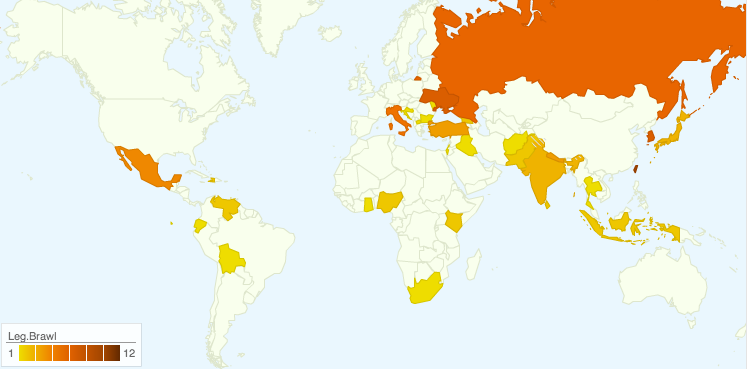
\includegraphics[width = 13cm]{incidence_map.png}
\end{figure}

%%%%%%%%%%%%%% Describing violence in National Legislatures
\section{Describing Violence in National Legislative Chambers Around the World (1981-2011)}

In order to further systematically explore the causes of legislative violence across the contemporary globe I used the Google News Archive\endnote{See {\url{http://news.google.com/archivesearch}}.} to create a data set of {\emph{physical fights between legislators in national legislative chambers}}.\endnote{The Google News Archive search was conducted in Spring 2011. Please contact me for a complete list of sources and search terms.} This resulted in a data set of 88 incidence of legislative violence in 30 countries between 1981 and Winter 2011. We can see in Figure \ref{leg_map} that these events have occurred in many regions around the world. They do not appear to be confined to any one cultural group or region as a simple regional culture explanation would predict. Violence is nonetheless not evenly distributed across countries. I observed 30 countries having legislative violence, but over 60 percent of these fights occurred in eight countries with four or more total legislative brawls. These countries include Ukraine, Mexico, South Korea, and Taiwan. 

Before moving on to the regression analysis it is useful to first examine the simple associations between proportional electoral outcomes, democratic age, and violence in this data. Figure \ref{framework_empirical} plots variables measuring these concepts in the entire sample of countries. In the following parametric analysis we will only look at multi-party elected legislatures. Each point represents a country-year. It's notable that all of the observed incidence of violence took place in legislatures with more disproportionate seat distributions.\endnote{Disproportionality is measured with the Gallagher disproportionality score \citep[][see the discussion below for further details]{Gallagher1991,Gallagher2012}.} Similarly, older democracies (approximately 55 years or older)\endnote{Democratic age is determined by how many years in a row a country had Polity IV scores greater than 5. Five is the qualitative point the creators of the Polity data set chose for determining if a country is democratic or not \citep{Marshall2009}.} were never observed having legislative brawls.\endnote{This is not to say that physical fights between legislators never happen in these countries. For example, during the writing of this paper a member of the United Kingdom Parliament assaulted a number of people at a Palace of Westminster pub. See {\url{http://www.guardian.co.uk/politics/2012/mar/12/eric-joyce-labour-membership}}.} 

While it appears that having disproportionate electoral outcomes \emph{or} a new democracy is not necessary for legislative violence, based on the data, having \emph{both} of them might make violence much more likely. South Korea's national assembly, like the antebellum US Senate, is an example of a `perfect storm'. It has both a new democracy and relatively disproportionate electoral outcomes.\endnote{South Korea’s average disproportionality as measured by the Gallagher Index from 2000 until 2011 was 12.7. This places it in the upper 25 percent of observations with elected legislatures. It also became a democracy within the past 20 years.} South Korea had eight observed incidence of legislative violence in the full sample. Countries that have \emph{either} proportional outcomes \emph{or} old democracies appear to be able to compensate for an absence of the other characteristic. The United Kingdom has a fairly disproportionate electoral system,\endnote{It had an average Gallagher disproportionality of 16.5 from 2000 to 2011.} but no violence in the sample. One reason for this might be that it has a very old democracy where both left-leaning Labour and right-leaning Conservative parties have had experience in government and so view commitments to allow for the alteration of power to be credible.  Conversely, no violence was observed in South Africa's new democracy--which is about the same age as South Korea's--but has very proportionate electoral outcomes.\endnote{South Africa’s average disproportionality was 0.29 from 2000 until 2011, one of the lowest observed in the sample.} So it may be easier for legislators to make credible commitments.

This brief tour of descriptive statistics adds to the evidence from the previous case study suggesting that violence between legislators does not occur randomly or is confined to one cultural region. Instead violence does appear to be a characteristic of countries with disproportionate electoral outcomes and new democracies.

%%%%%%%%%%%%%%%% Scatterplot of Disproportionality, AgeDem, and Violence %%%%%%%%%%%%%%%%%%%%%%%%
\begin{figure}[t]
    \caption{Scatter plots of Disproportionality, Age of Democracy, and Violence in the Full Sample.}  
    \label{framework_empirical}
    \begin{center}

\begin{knitrout}
\definecolor{shadecolor}{rgb}{0.969, 0.969, 0.969}\color{fgcolor}
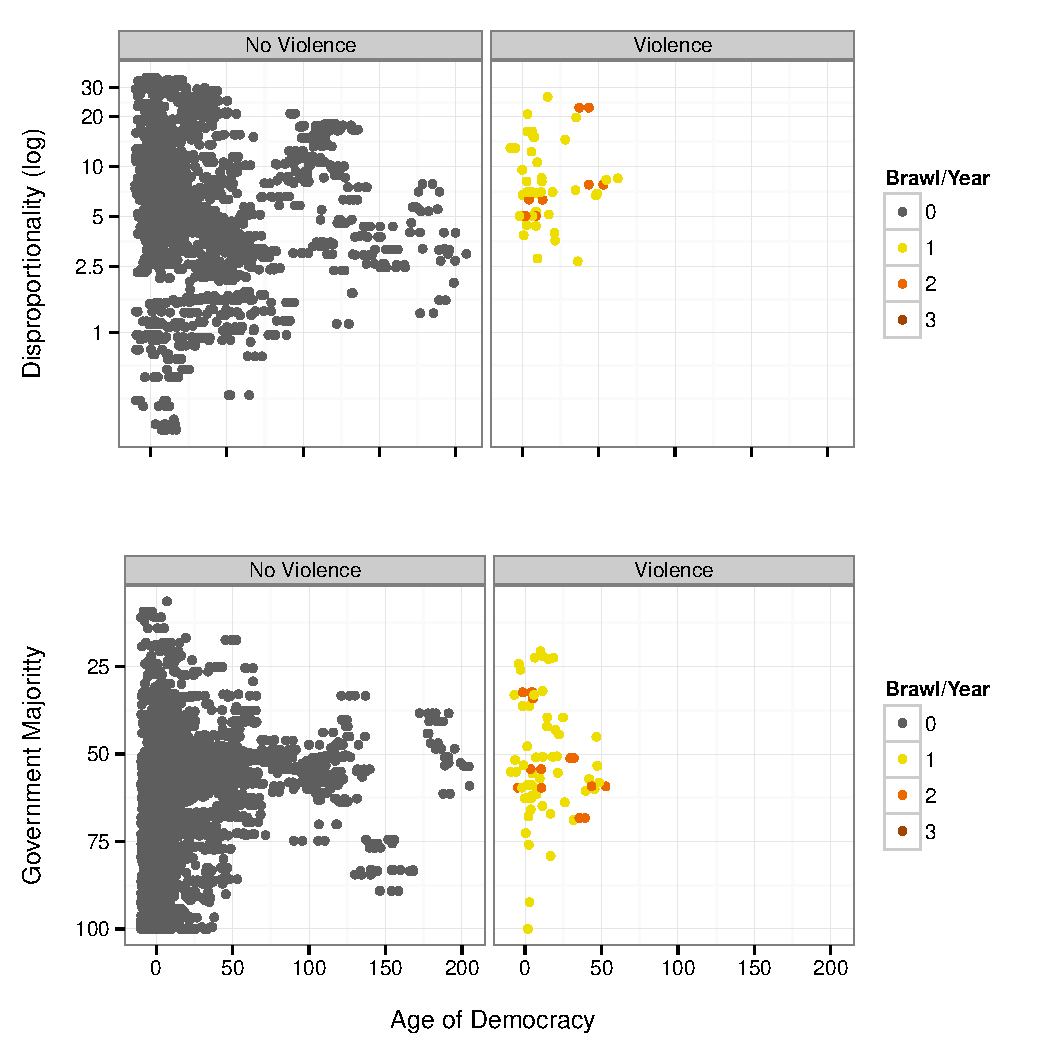
\includegraphics[width=0.8\linewidth]{figure/FrameworkEmpirical} 

\end{knitrout}

    \end{center}
    \begin{singlespace}
        {\scriptsize{Each point represents a country-year. \\ The data is from a sample of 200 countries between 1981 and 2009 due to data availability. The points are jittered horizontally to make them easier to see.}}
    \end{singlespace}

\end{figure}

%%%%%%%%%%%%%%%% Run Analyses %%%%%%%%%%%%%%%%%%%%%%%%



%%%%%%%%%%%%%%%%%%%%%%%%%%%%%%%%%%%%%%%%%%%%%%%%%%%%%%%%%%%%%%%%%%%%%%%%%%% Empirical Analysis
\section{Parametric Analysis: Set up}

To more closely and robustly investigate these findings I use incidences of legislative brawls in multi-party elected legislative chambers per country-year\endnote{Country-years with more than one act of violence are given multiple records. See below for a discussion of how the standard errors were adjusted to address statistical issues related to this.} as the dependent variable in a series of rare events logistic regression models \citep{KingRareEvents2001, KingRareEventsPA2001}. All country-years for which data is available over the observation period, regardless of legislative violence, are included in the sample. Data on whether or not a legislature had multiple elected parties is from the Database of Political Institutions (DPI) \citep[updated to 2010]{DPI2001} {\emph{Legislative Indices of Electoral Competitiveness}} variable.\endnote{Specifically, I kept only elected legislatures that DPI codes as having elections where multiple parties won seats, i.e. an LIEC score of 6 or 7.} Due to a lack of data on some of the co-variates discussed below, I also constricted the sample to years before 2010. This reduced the number of legislative violence incidences from 88 to 69. Full replication data and code used for all of the analyses can be found in this paper's source code files.\endnote{Full replication files can be found at \url{https://github.com/christophergandrud/LegislativeViolence}.}

%%%%%%%%%%%%%%%%%%%%%%%%%%%%%%%%%%%%%%%%%%%% Empirical Model
\subsection{Parametric Model: Rare Events Logistic Regression}

Legislative brawls are rare. Most of the time the overwhelming majority of legislatures do not have physical fights. The rarity of legislative brawls creates some empirical problems. Standard logistic regression techniques can ``sharply underestimate the probability of rare events" \cite[137]{KingRareEventsPA2001}. Estimated regression coefficients from logistic regression analysis with many fewer observed events than non-events will be too small. Furthermore, standard methods for computing event probabilities with logistic regression produce results biased in the same direction as the coefficient estimates. To overcome this problem \cite{KingRareEvents2001,KingRareEventsPA2001} propose a bias-corrected logistic model for rare events data--rare events logistic regression. I use this method below.\endnote{If there is no rare event bias, rare events logistic regression will produce results similar to a standard logit analysis. Please see King and Zeng \citep[147--148]{KingRareEventsPA2001} for a more detailed discussion of $\mathrm{Bias}(\hat\beta)$.}

%%%%%%%%%%%%%%%%%%%%%%%%%%%%%%%%%%%%%%%%%%%% Independent variables
\subsection{Right-hand Variables}

I included a number of political, societal, and economic variables in the regression models to test if the associations we saw earlier are actually spurious. Variable descriptions and sources are summarized in Table \ref{var_summary} in the Appendix. In the interest of transparency, the table includes all of the variables that I have included in all versions of the models, even those not shown because they did not generate substantively or statistically meaningful results.\endnote{Estimates from a number of them are not shown for simplicity. In general, these variables that are not shown in the following results tables did not generate statistically significant results and it was theoretically unclear how they would influence legislative violence. Nonetheless, please contact me for these results tables.} A matrix illustrating the variables' correlations can be found in Figure \ref{corrmatrix} in the Appendix. This figure also includes the variables' observed minimum and maximum values for reference. 

I measure the {\emph{age of a democratic regime}} as the number of years a country's Polity IV score is greater than five, the point above which that data set's creators classify a country as democratic. I use two variables to examine the relationship between the proportionality of electoral outcomes and violence. One is purely institutional: a simple dummy of whether or not a country's legislatures are elected by some form of {\emph{proportional electoral system}}. The variable is from the DPI database. As noted earlier, simply looking at the electoral mechanics confuses mechanisms with outcomes. So, more importantly, I use the standard Least Squares or Gallagher Index \citep{Gallagher1991} to measure realized {\emph{electoral disproportionality}}.\endnote{Carey and Hix refer to the Index as the ``established means of measuring proportionality in electoral systems" \citeyearpar[387]{Carey2011}. The index is calculated for each election with the following equation: $ \mathrm{LS} = \sqrt{\frac{1}{2}\displaystyle\sum_{i=1}^{n} (v_{i}-S_{i})^2}$, where $V_i$ is the vote share for party $i$ and $S_{i}$ is party $i$'s seat share. The available data is in terms of overall national disproportionality} To gain maximum coverage, I compiled the data from both \cite{Gallagher2012} and \cite{Carey2011}.\endnote{Full details can be found at {\url{http://christophergandrud.github.com/Disproportionality_Data/}}.} A country's disproportionality score is treated as constant from the year of an election until the year before the following election. Higher values on the Gallagher Index indicate more disproportionate, i.e. less fair electoral outcomes. 

As we saw in Figure \ref{framework_empirical} there appears to be a very strong negative correlation between very low levels of disproportionality and legislative violence. No instances of violence were observed in countries with a disproportionality score of less than about 2.5.\endnote{Though the observed range of disproportionality scores goes from almost 0 to 30, countries with scores less than 2.5 are not outliers. About 42 percent of county-years in the sample had scores of 2.5 or smaller.} This can be explained by fairness equilibria and is partially corroborated by Marien's \citeyearpar{Marien2011} finding regarding very low disproportionality measured with the Gallagher Index and political trust discussed above. To capture a possible disproportionality threshold effect--where low disproportionality is associated with stronger feelings of fairness--I created a low disproportionality dummy variable. County-years with disproportionality greater than or equal to the observed median (6)\endnote{The observed range is 0.26 to 34.52.} are coded as having higher disproportionality and those with scores lower than 6 are coded as having lower disproportionality.\endnote{Models were estimated with the continuous disproportionality measure. The parameter estimates were not statistically significant and are not shown.} 

I also investigated the possibility that a number of political, institutional, and cultural variables may actually be associated with legislative violence and that the key variables from my argument actually have spurious associations. To get a sense of how the size of the governing majority is associated with legislative violence I include the government {\emph{majority}} variable (from the DPI). It simply measures the seats held by governing parties as a proportion of all seats. I transformed the variable from a proportion to a percentage to ease interpretation. Legislators may be less likely to attack one another if they know that they could be arrested for assault. To examine this possibility I include Fish and Koening's \citeyearpar{Fish2009} dichotomous \emph{legislator immunity} variable. It equals one if national legislators are immune from arrest and/or prosecution and zero otherwise. Unfortunately, their data only captures legislative immunity in 2007. I extrapolated the 2007 value of the variable to the other observation years.\endnote{I also considered using the legislator immunity variable from the Comparative Constitutions Project \citep{ElkinsCCP2010}. However, the coding of the immunity variable is vaguer than Fish and Koening's and only deals with constitutionally mandated immunity.} We should therefore approach results from this variable with some caution since it might not be a valid indicator for all country-year observations.

To examine the relationships between societal-level values and legislative violence I rely primarily on data from the World Values Survey \citeyearpar{WVS2009}. Over the course of his research, Ingelhart has found that his composite {\emph{self-expression}} indicator is the best way to capture cultural and normative differences between democracies and non-democracies. Societies have high self-expression scores if they emphasize ``liberty and participation, public self-expression, tolerance of diversity, interpersonal trust, and life satisfaction" \citep[64]{Inglehart2003}. So I include the self-expression variable from the World Values Survey.\endnote{In earlier versions of the models I also included components of this variable. However, they were either never statistically significant or produced unintelligible and unstable results.} Following \cite{Inglehart2003} I average the variables across individual participants within countries and survey waves. I only use the third through fifth survey waves\endnote{The surveys were taken in the following years: \\ Wave 3: 1994--1998 \\ Wave 4: 1999--2004 \\ Wave 5: 2005--2007} as the first two waves have very poor coverage. I used wave 3 for all years before 1998, wave 4 for all years between 1999 and 2004 and wave 5 onward. 

To assess any effect of coalition compared to single-party governments I included the DPI {\emph{government fractionalization}} variable. It is the probability that two randomly picked deputies in the government are from different parties. I used the fractionalization variable to create an indicator of {\emph{single-party}} government. It is simply a dummy equalling one if fractionalization was zero, i.e. all governing legislators were from the same party. In general single party governments probably are better able to pass policies very close to their ideal preferences. This could heighten losers' losses and make them less likely to want to conform to non-violent legislative rules. However, all single party governments are not created equal. Some parties may act as umbrella parties that incorporate many different factions. While others are narrowly focused on a particular constituency. 

I also included standard measures of the \emph{effective number of parliamentary parties} by votes and by seats \citep[see][]{Laakso1979, Taagepera1989}. The data was taken from \cite{Carey2011}\endnote{Their data is mostly from \cite{Golder2005}. Please see their notes for further details.} before 2004 and from \cite{Gallagher2012} afterwards. Both of these measures indicate how fragmented a parliamentary party system is. Higher scores indicate that there are more parties that win either votes or seats. Neither measure produced statistically significant results, so only the results for the effective number of parties by seats are shown below.

To examine whether or not national legislative losers may be dissuaded from legislative violence because there is a possibility of gaining power at a provincial-level, I include the \emph{federalism} dummy variable from \cite{Carey2011}.\endnote{Their data is mostly from \cite{Adsera2003}. Please see their notes for further details.} I updated this from 2004 until the end of the observation period. In early models I also controlled for the government system type, i.e. if it had a presidential, parliamentary, or mixed assembly-elected presidential. This was from the DPI.

I include a number of other societal-level variables to help further defend against omitted variable bias. Conflict in more ethnically or economically divided societies may be generally more intense. These conflicts may spill over into legislatures where they precipitate violence between members. I include Alesina et al.'s \citeyearpar{Alesina2003} {\emph{ethnic fractionalization}} data to account for the fact that a legislature's composition in terms of its fractionalization is not only a function of political institutions, but also social divisions \citep{Neto1997, Mozaffar2003}. The variable measures the probability that two randomly selected members of society will be from different ethnic groups. Higher values indicate more societal fractionalization. To capture similar possible effects from economic divisions, I include {\emph{Gini coefficients of economic inequality}} from \cite{UNU2008}.\endnote{Note, for country-years with missing data I assumed that the Gini Coefficient remained constant from the last year there is data for the country, unless the span was ten years or more. If this was the case they were treated as missing.} Finally, as is common in cross-country analyses, I also include {\emph{gross domestic product per capita}}. This data is from the World Bank's International Development Indicators \citeyearpar{WorldBank2011} and is in thousands of United States dollars.

%%%%%%%%%%%%%%%%%%%%%%%%%%%%%%%%%%%%%%%%%%%% Analyses


\section{Rare Events Logistic Regression Results}

I used the {\tt{relogit}} model from the {\tt{R}} package Zelig \citep{IMAIKingZelig2008} to estimate the rare events bias corrected logit regression models. Furthermore, to get a better understanding of the magnitude of the estimated relationships between the right-hand variables and violence, I also used Zelig to predict incident probabilities with 1000 simulations per fitted value \citep[see][]{King2002}. Predicted probabilities for various fitted values of the key findings of interest with robust results are shown in Figure \ref{pred_prob}. These give us a substantively meaningful sense of estimated effects' magnitudes. Note: because the variables are recorded in country-year records, all of the results should be interpreted in terms of the predicted effect of a variable on the probability of legislative violence in a given country in a year. Regression coefficient point estimates and robust standard errors can be found in tables \ref{outputTable.dem} and \ref{outputTable.1990}.

I observed relatively few incidences of violence in the 1980s.\endnote{There were only 8 observed incidence before 1990.} This may be because news articles from before the 1990s have not been made available on the internet with the same frequency as those written from the 1990s. To examine any estimation biases this sampling bias might create I ran the regressions on a further constricted sample of multi-party elected legislatures from 1990.\endnote{For prior correction in the full sample of competitively elected legislatures I used the existing proportion of all observations with legislative violence in the time constricted sample 1.7 percent of observations up until 2010 had violence ($\tau = \frac{69}{3347} = 0.021$). for prior correction in the rare events logistic regressions \citep[see][]{KingRareEventsPA2001}. I used the observed number of violent incidences from 1990. There were 61 observed incidences of violence and 2778 country-years from 1990 through 2009 in the sample, so: $\tau = \frac{61}{2531} = 0.023$.} The results were broadly similar across the two samples. 

Individual observations are clearly correlated within countries and years, especially when there were multiple acts of violence in a country in a year. To address this issue I used robust standard errors \citep{Golder2006, Mainwaring2007}. Standard errors were adjusted using \cite{Lumley1999} weighted empirical adaptive variance estimators (WEAVE) where the true dependence structure does not need to be specified prior to running the analysis.\endnote{Also, using WEAVE to find robust standard errors allowed me to take advantage of Zelig's ability to simulate quantities of interest. Results were very similar to those from estimating the same models in Stata using {\tt{relogit}} with the {\tt{cluster(country)}} option. Please contact me for tables comparing the two sets of results.} 

%%%%%%%% Elected Legislatures Results Table
\begin{table}
\caption{Legislative Violence Rare Events Logistic Regression Results (Multi-Party Elected Legislature 1981-2009)}
\label{outputTable.dem}
\begin{center}

\begin{tabular}{l c c c c c c }
\hline
                        & A1 & A2 & A3 & A4 & A5 & A6 \\
\hline
(Intercept)             & $-3.04^{***}$ & $-1.15$       & $-6.75$      & $-1.00$       & $-1.44$      & $-1.46$      \\
                        & $(0.20)$      & $(0.79)$      & $(5.45)$     & $(0.62)$      & $(0.79)$     & $(0.96)$     \\
Low Disproportionality  & $-1.00^{**}$  & $-1.43^{***}$ & $-2.26^{**}$ & $-1.28^{***}$ & $-1.22^{**}$ & $-1.02^{**}$ \\
                        & $(0.35)$      & $(0.37)$      & $(0.75)$     & $(0.38)$      & $(0.38)$     & $(0.37)$     \\
Dem. Age                & $-0.02^{*}$   & $-0.02^{*}$   & $-0.02$      & $-0.02^{**}$  & $-0.02^{**}$ & $-0.02$      \\
                        & $(0.01)$      & $(0.01)$      & $(0.01)$     & $(0.01)$      & $(0.01)$     & $(0.01)$     \\
Majority Size           &               & $-0.04^{***}$ & $-0.04^{*}$  & $-0.04^{***}$ & $-0.03^{**}$ & $-0.03^{**}$ \\
                        &               & $(0.01)$      & $(0.02)$     & $(0.01)$      & $(0.01)$     & $(0.01)$     \\
Leg. Immunity           &               & $-0.48$       &              &               &              &              \\
                        &               & $(0.34)$      &              &               &              &              \\
PR Electoral System     &               & $1.02^{*}$    &              &               &              &              \\
                        &               & $(0.51)$      &              &               &              &              \\
Single Party Gov.       &               & $-0.43$       &              &               &              &              \\
                        &               & $(0.32)$      &              &               &              &              \\
Self Expression         &               &               & $4.62$       &               &              &              \\
                        &               &               & $(4.20)$     &               &              &              \\
Ethnic Frac.            &               &               & $0.50$       &               &              &              \\
                        &               &               & $(1.17)$     &               &              &              \\
Federal                 &               &               &              & $0.96^{*}$    & $0.93^{*}$   &              \\
                        &               &               &              & $(0.38)$      & $(0.40)$     &              \\
Gov. Frac.              &               &               &              & $0.36$        &              &              \\
                        &               &               &              & $(0.56)$      &              &              \\
No. of Parties by Seats &               &               &              &               & $0.08$       &              \\
                        &               &               &              &               & $(0.09)$     &              \\
GINI                    &               &               &              &               &              & $0.00$       \\
                        &               &               &              &               &              & $(0.02)$     \\
GDP per Capita          &               &               &              &               &              & $0.01$       \\
                        &               &               &              &               &              & $(0.03)$     \\
\hline
AIC                     & 408.22        & 390.07        & 185.71       & 357.36        & 336.71       & 361.87       \\
BIC                     & 424.88        & 428.82        & 213.07       & 389.98        & 369.15       & 394.57       \\
Log Likelihood          & -201.11       & -188.03       & -86.86       & -172.68       & -162.35      & -174.94      \\
Deviance                & 402.22        & 376.07        & 173.71       & 345.36        & 324.71       & 349.87       \\
Num. obs.               & 1905          & 1873          & 706          & 1697          & 1649         & 1718         \\
\hline
\multicolumn{7}{l}{\scriptsize{\textsuperscript{***}$p<0.001$, 
  \textsuperscript{**}$p<0.01$, 
  \textsuperscript{*}$p<0.05$}}
\end{tabular}



\end{center}
{\scriptsize{
    Standard errors are in parentheses. All models use robust (WEAVE) standard errors. \\
}}
\end{table}

%%%%%%%% Elected Legislatures Results Table from 1990
\begin{table}
\caption{Legislative Violence Rare Events Logistic Regression Results (Multi-Party Elected Legislature from 1990-2009)}
\label{outputTable.1990}
\begin{center}

\begin{tabular}{l c c c c c c }
\hline
                        & B1 & B2 & B3 & B4 & B5 & B6 \\
\hline
(Intercept)             & $-2.90^{***}$ & $-0.78$       & $-7.82$      & $-0.90$       & $-1.30$      & $-1.73$      \\
                        & $(0.22)$      & $(0.82)$      & $(5.72)$     & $(0.65)$      & $(0.85)$     & $(1.04)$     \\
Low Disproportionality  & $-0.86^{*}$   & $-1.19^{**}$  & $-2.03^{**}$ & $-1.18^{**}$  & $-1.10^{**}$ & $-0.96^{*}$  \\
                        & $(0.38)$      & $(0.39)$      & $(0.76)$     & $(0.40)$      & $(0.41)$     & $(0.40)$     \\
Dem. Age                & $-0.02^{*}$   & $-0.02^{*}$   & $-0.02$      & $-0.02^{*}$   & $-0.02^{*}$  & $-0.03^{*}$  \\
                        & $(0.01)$      & $(0.01)$      & $(0.01)$     & $(0.01)$      & $(0.01)$     & $(0.01)$     \\
Majority Size           &               & $-0.04^{***}$ & $-0.05^{**}$ & $-0.04^{***}$ & $-0.04^{**}$ & $-0.03^{**}$ \\
                        &               & $(0.01)$      & $(0.02)$     & $(0.01)$      & $(0.01)$     & $(0.01)$     \\
Leg. Immunity           &               & $-0.29$       &              &               &              &              \\
                        &               & $(0.37)$      &              &               &              &              \\
PR Electoral System     &               & $0.64$        &              &               &              &              \\
                        &               & $(0.53)$      &              &               &              &              \\
Single Party Gov.       &               & $-0.45$       &              &               &              &              \\
                        &               & $(0.35)$      &              &               &              &              \\
Self Expression         &               &               & $5.94$       &               &              &              \\
                        &               &               & $(4.45)$     &               &              &              \\
Ethnic Frac.            &               &               & $0.54$       &               &              &              \\
                        &               &               & $(1.36)$     &               &              &              \\
Federal                 &               &               &              & $0.79$        & $0.72$       &              \\
                        &               &               &              & $(0.43)$      & $(0.47)$     &              \\
Gov. Frac.              &               &               &              & $0.49$        &              &              \\
                        &               &               &              & $(0.61)$      &              &              \\
No. of Parties by Seats &               &               &              &               & $0.09$       &              \\
                        &               &               &              &               & $(0.09)$     &              \\
GINI                    &               &               &              &               &              & $0.02$       \\
                        &               &               &              &               &              & $(0.02)$     \\
GDP per Capita          &               &               &              &               &              & $0.03$       \\
                        &               &               &              &               &              & $(0.03)$     \\
\hline
AIC                     & 338.58        & 325.93        & 148.72       & 292.94        & 271.91       & 299.07       \\
BIC                     & 354.46        & 362.88        & 174.56       & 324.02        & 302.75       & 330.29       \\
Log Likelihood          & -166.29       & -155.96       & -68.36       & -140.47       & -129.95      & -143.53      \\
Deviance                & 332.58        & 311.93        & 136.72       & 280.94        & 259.91       & 287.07       \\
Num. obs.               & 1473          & 1450          & 548          & 1313          & 1262         & 1344         \\
\hline
\multicolumn{7}{l}{\scriptsize{\textsuperscript{***}$p<0.001$, 
  \textsuperscript{**}$p<0.01$, 
  \textsuperscript{*}$p<0.05$}}
\end{tabular}


\end{center}
{\scriptsize{
    Standard errors are in parentheses. All models use robust (WEAVE) standard errors. \\
}}
\end{table}

I avoid focusing on models that include highly correlated variables \citep[see][]{Achen2002, Schrodt2006}. In these models (not shown), as the statistical literature predicts, the coefficient estimates and standard errors change dramatically for many of the variables. There may be interactions between many of the variables included in the models. I attempted to capture interactions in the analysis, but it was empirically difficult. Given the small number of observed incidences of legislative violence there could simply not be enough information in the data to draw meaningful conclusions about these types of relationship \citep[see][]{Brambor2006}. I also ignore results from models with the government system type variable. It had very large, highly unstable, and largely nonsensical coefficient estimates, suggesting that the model does not contain enough information to test \citep{Babyak2004} whether or not political system type has an effect on violence.

%%%%%%%%%%%%%%%% Predicted Probability Graphs %%%%%%%%%%%%%%%%%%%%%%%%
\begin{figure}[t]
    \caption{Predicted Probability of Legislative Violence in Multi-Party Elected Legislatures}  
    \label{pred_prob}
    \begin{center}

    %\includegraphics[width = \textwidth]{leg_violence_paper-PredProb}

\begin{knitrout}
\definecolor{shadecolor}{rgb}{0.969, 0.969, 0.969}\color{fgcolor}
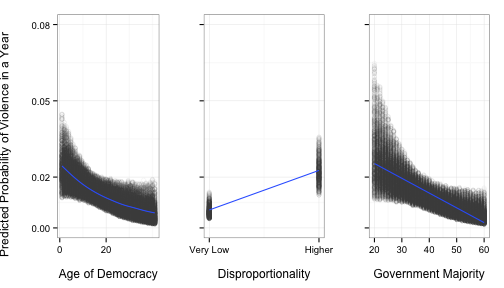
\includegraphics[width=0.8\linewidth]{figure/predProb} 

\end{knitrout}

    \end{center}
    \begin{singlespace}
      {\scriptsize{The graphs show the middle 95\% of 1000 simulations at each fitted value of the variables. The simulations use Model B2 with the sample constricted to observations from 1990. See Table \ref{outputTable.1990}. For each set of simulations all other variables were fitted at their means.}}
    \end{singlespace}
\end{figure}

\paragraph{Disproportionality}

Across all of the models the estimates for the dummy {\emph{low disproportionality}} variable indicate that very proportional electoral outcomes are associated with less legislative violence. This finding is robust\endnote{It is statistically significant at least at the 5\% significance level.} in all model specifications. The finding confirms what we saw in Figure \ref{framework_empirical}. Violence is very rare in countries with Gallagher scores below the median--6--and there is something of a cut-off point--around 2.5--below which these highly proportional countries were not observed to have had any violence. More interesting than simple statistical significance or coefficient point estimates is the magnitude of and uncertainty surrounding the disproportionality/violence relationship. To get a sense of the magnitude of this estimated relationship and the uncertainty around it \citep[see][]{King2000} I plotted the predicted probabilities of having a legislative brawl in the left-most plot of Figure \ref{pred_prob} using information from Model B2 with the sample constricted to observations from 1990.\endnote{To estimate these probabilities I ran 1000 simulations for each value of the low disproportionality variable using estimates from model B2. Other covariates were held at their means.} We can see that the predicted probability that a country will have violence when disproportionality is greater than or equal to 6 is a little over two percent in a given year, fitting all other variables at their means. Countries with disproportionality less than 6 had almost no predicted probability of violence in a year.

\paragraph{Age of Democracy}

Also, corroborating what we saw in Figure \ref{framework_empirical}, the rare events logit analyses indicate that older democracies tend to have less legislative violence. This result is significant at at least the 10 percent level in all of the models. Looking at the middle panel of Figure \ref{pred_prob} we can see that violence is more likely in younger democracies. Very young democracies are predicted to have about a two percent probability of experiencing legislative violence in a given year. This is a similar magnitude to that estimated for countries with higher disproportionality. The probability of violence decreases steadily as a democracy ages. The predicted probability of violence becomes largely indistinguishable from zero--i.e. no probability of violence--sometime shortly after a democracy turns 50 years old.

\paragraph{Governing Majorities}

I also found a negative relationship between the size of governments' legislative majorities and violence. We can see in the right-most panel of Figure \ref{pred_prob} that the predicted probability of violence in countries with minority governments is relatively high at slightly over 5 percent in a year. This is somewhat higher than predicted for countries with high disproportionality or new democracies, though the variance is much larger. This finding fits well within this paper's main argument. Non-legislative cartel members likely view the minority's control of the agenda as unfair--even if the minority government has a constrained ability to affect policy change--and may see considerable opportunities to shift power in their direction. They would be less able to make credible commitments. The minority government may at the same time use violence to try to block attempts to increase fairness. This could make it more difficult for both sides to credibly commit. 

It is still less theoretically clear what is causing the very low probability of violence in large majority countries. It could be that legislators in these parliaments view the decisions of the larger majority as more legitimate or it could be that hegemonic parties are able to effectively quash disruption and violence before it starts. It is difficult to separate out these two possible causes here. I did try to rule out the possibility that the result is being driven by legislatures with very powerful parties that control virtually all of the seats. To do this I reran the models where observations with government majorities greater than or equal to 75 percent were dropped. The results (not shown) nonetheless persisted.\endnote{Please contact the author for these results tables.} Further case study work is needed to understand the causes of a lack of violence in legislatures with large majorities.

\paragraph{Cultural and Societal Variables}

None of the cultural, ethnic fractionalization, or other societal-level variables such as the GINI coefficient and GDP per Capita were found to be associated with legislative violence in any of the models. In some limited models (not shown) with data from 1990 ethnic fractionalization was negatively associated with violence. However, the effect became statistically insignificant whenever high disproportionality was included in the models. We should be somewhat sceptical about the strength of the conclusions we can draw from the self-expression variable results. As mentioned early there might be a highly endogenous relationship between culture and institutions. However, if culture was driving institutions that were associated with legislative violence, presumably the cultural variables would have also been associated with violence in models without the institutional variables, which they were not. Nonetheless, it takes a bit of a leap to believe that the mean level of self-expression found using a national-level survey accurately reflects the values held by elite individuals in legislatures. Further work is needed to make stronger conclusions about the relationships between culture and the propensity for legislative violence. This research could possibly use individual legislator-level surveys that would allow us to directly measure the distribution of values among actual legislators. At this point we can say that we have not yet found evidence that national-level cultures and divisions are strongly associated with a propensity for violence.

\paragraph{Other Political and Institutional Variables}

Results for other political and institutional variables were largely not statistically significant. Legislative immunity from arrest and/or prosecution is not significantly associated with legislative violence. We should approach this result cautiously since the Fish and Koening immunity variable is based on observations in 2007 and therefore might not be a valid indicator for many country-years. The observed positive relationship between proportional electoral systems and violence, though seemingly counter-intuitive, was not robust across the models. This fits with the argument that we should focus on electoral outcomes rather than simple mechanics. Neither effective number of parties variables, the basic continuous government fractionalization variable, nor the single-party government variable were statistically significant in the analyses. Likewise, federalism did not appear to be robustly related to legislative violence across the models. All of these variables are not as directly related to legislators' sense of fairness and an ability to make credible legislative commitments at a theoretical level, compared to disproportionality, democratic age and, to a lesser extent, governing majority size. So it should not come as too much of a surprise to find that they are more loosely, if not at all, associated with legislative violence.

%%%%%%%%%%%%%%%%%%%%%%%%%%%%%%%%%%%%%%%%%%%% Conclusions
\section*{Conclusions: What Keeps Legislators Two Sword Lengths Apart?}

In this paper--the first to systematically examine legislative violence in multi-party elected legislative chambers on a global scale--I developed an argument that violence in these chambers is more likely when legislators are unable to make credible commitment to peaceful bargaining outcomes, including non-violent legislative rules. This problem greatly exacerbated by a lack of legislative fairness. I then empirically tested my argument with a case study of the canning of Senator Sumner in the antebellum United States and a new data set of legislative brawls. What conclusions can we make from the paper's findings about why legislators are kept `two sword lengths' apart (or not) and what implications do they have?

The findings in this paper suggest that countries with highly proportional--very fair--electoral outcomes rarely experience legislative violence. It's notable that violence in antebellum United States occurred in the Senate, which was much more disproportional than the House of Representatives. Looking more broadly at the recent global sample the relationship appears to be subject to a threshold effect where countries with Gallagher Index scores below about 6 rarely experience legislative violence and those below 2.5 never did. This corresponds closely to the idea of a fairness equilibrium and previous findings made by Marien \citeyearpar{Marien2011} about perceptions of political trust in countries with highly proportional outcomes using the same measure. 

The proportionality finding is further illustrated by new Southern African democracies, chiefly South Africa and Namibia. Despite having new democratic institutions, very fractious societies, and recent histories of intense armed conflict, neither country was recorded to have experienced legislative violence.\endnote{This does not mean that there are no instances of disruption in these legislatures. However, disruption has always been non-violent \cite[for research on South Africa see][]{Johnson2013}.} Since transitioning to democracy they had highly proportional electoral outcomes.\endnote{Namibia's average disproportionality for its years as a democracy is 0.83 and South Africa's is 0.31. South Africa has one of the most proportional systems in the sample.}   

This finding is perhaps more important than the paper's age of democracy result for democratic institutional designers who may want to actively keep legislators two sword lengths apart. Democratic age is subject to many factors far outside of the control of democratic planners. Electoral disproportionality is comparatively much more malleable. Proportional electoral systems are the most obvious tool electoral system designers have to increase the correspondence between party's votes and seats \citep{Carey2011}. These systems can be tweaked by increasing district magnitude or altering the formula used to translate votes into seats depending on the distribution of preferences in the electorate. The findings in this paper suggest that electoral system designers may want to aim for very proportional outcomes in order to prevent violence in new democratic legislatures. 

As this is the first large scale study on this subject there is still considerable work that can be done to better understand the causes and consequences of legislative violence. As mentioned earlier more work is needed on legislator-level cultural values and the effects of very large majority governments. Further case study work could examine non-electoral fairness problems that could exacerbate credible commitment problems. Similarly, more research could be done on post-election solutions that make the distribution of legislative resources more fair \cite[for example see][who examined informal minority party access to power in Japan's Diet]{Wolfe2004}. Furthermore, what are the consequences of legislative violence, especially in terms of citizens' perceptions of democratic legitimacy and, indeed, the long-term viability of democratic regimes? These issues should be investigated in future work. 

%%%%%%%%%%%%%%%%%%%%%%%%%%%%%%%%%%%%%%% Appendix

\bibliographystyle{apsr}
\bibliography{LegViolence}

\theendnotes

%%%%%%%%%%%%%%%%%%%%%% Figures Start %%%%%%%%%%%%%%%%%%%%%%%%%%%%%%%%%%%%%%%%%%%%%

\clearpage
\section*{Appendix}


%%%%%%%% Variable source summary table
\begin{table}[!h]
    \begin{center}
    \caption{Variable Summary}
    \label{var_summary}
    \begin{tabular}{l m{7cm} m{3.5cm}}

            \hline
            Variable & Description & Source \\
            \hline \hline
            Disprop & Gallagher Index of Electoral Disproportionality & \cite{Gallagher2012} \& \cite{Carey2011} \\
            ENPS & Effective number of parties by seats & \cite{Gallagher2012} \& \cite{Carey2011} \\
            ENPV & Effective number of parties by votes & \cite{Gallagher2012} \& \cite{Carey2011} \\
            Ethnic Fractionalization & Probability two randomly selected members of society are from the same ethnic group & \cite{Alesina2003} \\
            Federal & Whether a country has a federal system or not & \cite{Carey2011}, updated from 2003 by the author \\           
            GDP/Capita & GDP per capita in thousands of US dollars & \cite{WorldBank2011} \\
            Gov. Fractionalization & Probability that two members of the Government will be from different parties & \cite{DPI2001} \\
            Gini & Gini Coefficient of income inequality & \cite{UNU2008} \\
            Immunity & Whether a legislators are immune from arrest and/or criminal prosecution or not & \cite{Fish2009} \\
            LEIC & Legislative Indices of Electoral Competitiveness. Includes both the existence of a legislature and its level of electoral competitiveness. & \cite{DPI2001} \\
            Majority & Percentage of legislature controlled by governing parties & \cite{DPI2001} \\
            Polity & Polity IV Score & \cite{Marshall2009} \\
            PR & Whether a country uses a proportional representation electoral system or a plurality system & \cite{DPI2001} \\
            Self Expression & WVS self-expression indicator averaged across country-survey waves & \cite{WVS2009} \\
            System & Government system (parliamentary, presidential, or mixed & \cite{DPI2001} \\
            Tenshort & Tenure of the shortest serving veto player & \cite{DPI2001} \\
            Trust & Average of WVS responses where 1 $=$ most people can be trusted and 2 $=$ you can't be too careful & \cite{WVS2009} \\
            UDS & Posterior Mean Unified Democracy Score & \cite{Pemstein2010} \\
            Violence & Incidences of violence between legislators in the national parliamentary chamber & author \\
            \hline

    \end{tabular}
    \end{center}
    \begin{singlespace}
        Please contact the author for detailed summary statistics. \\
        All of the data from \cite{DPI2001} was updated through 2010.
    \end{singlespace}
\end{table}  

%%%%%%%%%% Correlation matrix %%%%%%%%%% 
\begin{landscape}
\begin{figure}[t]
    \caption{Correlation Matrix for Variables Included in the Analysis (Multi-Party Elected Legislatures)}
    \label{corrmatrix}
    \begin{center}
    
    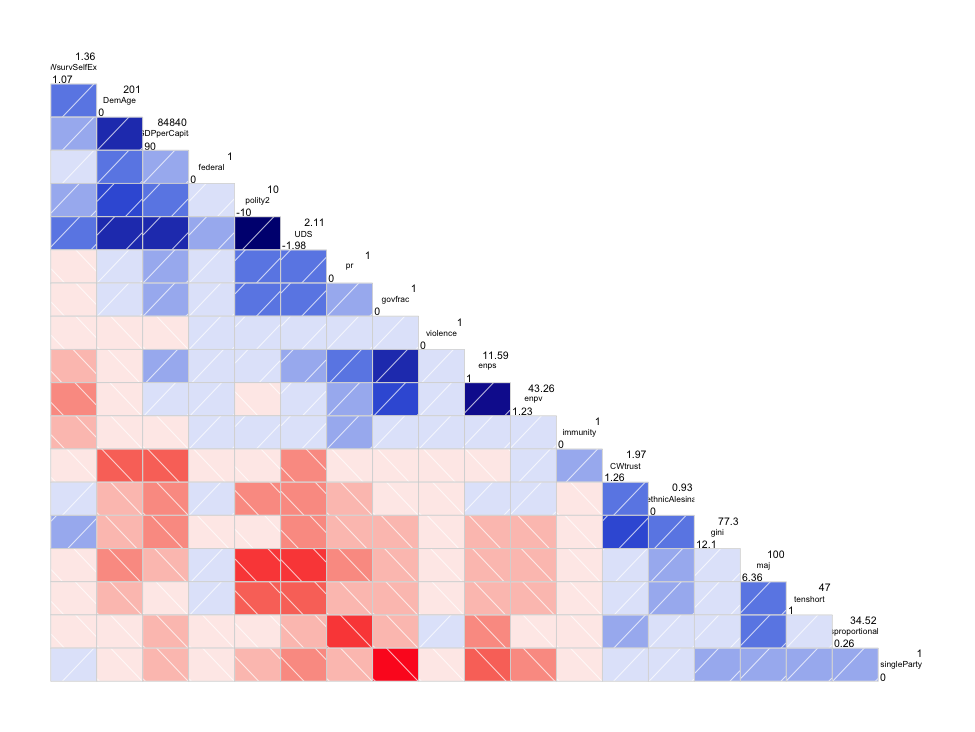
\includegraphics[width = \textwidth]{figure/corScatter.png}  
    %%% corScatter not created every compile to save time %%%
%<<corScatter>>=

%    library(corrgram)  

%    ### Create data set with variables for corrgram
%    vars.corrgram <- c("violence", "system", "DemAge", "maj", "MajCat", "govfrac", "singleParty", "pr", "tenshort", "UDS", "polity2", "ethnicAlesina", "CWtrust", "CWsurvSelfExpr", "disproportionality", "gini", "GDPperCapita", "enps", "enpv", "federal", "immunity")

%    # Subset elected legislature data
%    dem.corrData <- dem[vars.corrgram]

%    # Create corrgram
%    dem.corrgram <- corrgram(dem.corrData, order = TRUE, upper.panel = NULL, diag.panel = panel.minmax)

%@

    \end{center}
    \begin{singlespace}
        {\scriptsize{Redder squares indicate stronger negative bivariate correlations. \\
        Bluer squares indicate stronger positive bivariate correlations. \\
        Numbers in the diagonal squares indicate the minimum and maximum observed values of the variables in the sample.
        }}
    \end{singlespace} 
\end{figure}
\end{landscape}

%%%%%%%%%%%%%%%%%%%%%% Figures End %%%%%%%%%%%%%%%%%%%%%%%%%%%%%%%%%%%%%%%%%%%%%

\end{document}
